\begin{theorem}
    \label{teo:teorema_na}
    Sea $\alpha \notin \mathbb{Q}$ entonces la sucesión $(n\alpha)_{n\ge1}$ es equidistribuida módulo $1$.
\end{theorem}

\begin{proof} La demostración se basa en la observación~\ref{obs:equidistribucion}.

    Sea $(a,b) \in \mathbb{T}$, sea $\varepsilon > 0$ y sean $f_\varepsilon^-, f_\varepsilon^+ \in C(\mathbb{T})$
    funciones tales que 
    \[
       0 \leq 
       \mathbf{1}_{(a+\varepsilon, b-\varepsilon)} \leq 
       f_\varepsilon^- \leq 
       \mathbf{1}_{(a,b)} \leq 
       f_\varepsilon^+ \leq
       \mathbf{1}_{(a-\varepsilon, b+\varepsilon)} \leq
       1
    \]

    % No se si ve muy bien puede que lo quite.
    \begin{figure}
        \centering
        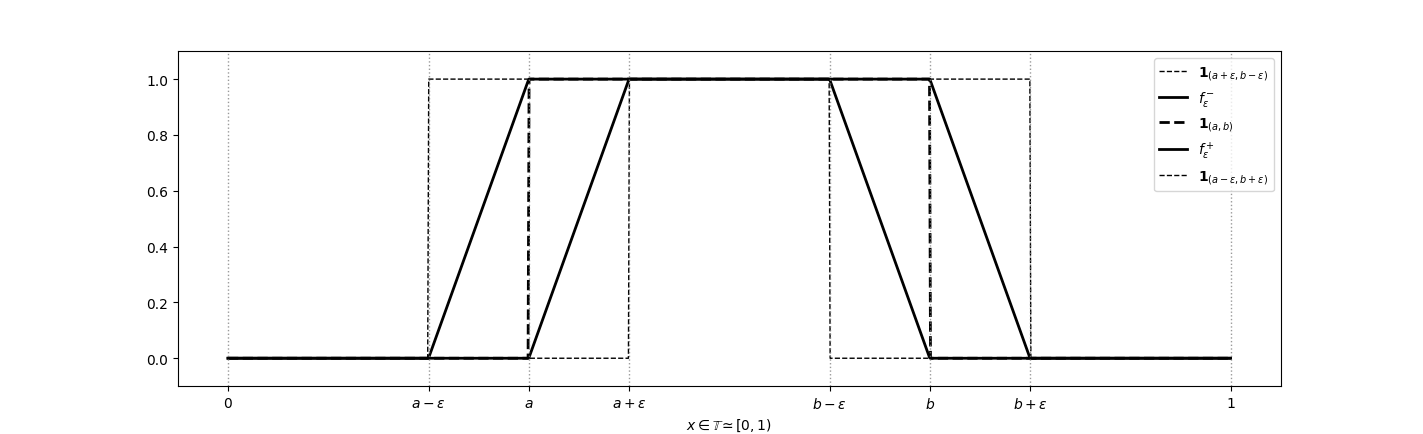
\includegraphics[scale=0.45]{pics/grafico_1_teorema_na.png}
        \caption{Gráfico de las funciones $\mathbf{1}_{(a+\varepsilon, b-\varepsilon)}$, 
        $f_\varepsilon^-$, $\mathbf{1}_{(a,b)}$, $f_\varepsilon^+$ y $\mathbf{1}_{(a-\varepsilon, b+\varepsilon)}$
        para el caso $(a,b) = (0.3, 0.7)$, $\varepsilon = 0.1$.}
    \end{figure}

    Sea $S_N = \sum_{n=1}^N \mathbf{1}_{(a,b)}(n\alpha)$, entonces,
    \[
        \frac{1}{N} \sum_{n=1}^N f_\varepsilon^-(n\alpha) \leq
        \frac{S_N}{N} \leq 
        \frac{1}{N} \sum_{n=1}^N f_\varepsilon^+(n\alpha)
    \]
    
    Por el lema anterior, se tiene que,
    \[
        b-a-2\varepsilon \leq
        \int_0^1 f_\varepsilon^-(x)\ dx \leq
        \liminf_{N \to \infty} \frac{S_N}{N} \leq
        \limsup_{N \to \infty} \frac{S_N}{N} \leq
        \int_0^1 f_\varepsilon^+(x)\ dx \leq
        b-a+2\varepsilon
    \]

    Finalmente, tomando el límite cuando $\varepsilon \to 0$ se obtiene,
    \[
        b-a \leq
        \liminf_{N \to \infty} \frac{S_N}{N} \leq
        \limsup_{N \to \infty} \frac{S_N}{N} \leq
        b-a
    \]

    Por lo tanto, el límite existe y
    \[
        \lim_{N \to \infty} \frac{1}{N} \sum_{n=1}^N \mathbf{1}_{(a,b)}(n\alpha) = b-a
    \]
\end{proof}